\section{RAVEN}
\label{sec:raven}
 
The Risk Analysis and Virtual ENviroment 
(RAVEN\footnote{Official website: \url{https://raven.inl.gov},\\ 
GITHUB repository: \url{https://github.com/idaholab/raven}})
~\cite{RAVEN_PSAM_2014,alfonsiEsrel2014} 
is a flexible and multi-purpose uncertainty quantification, regression analysis, probabilistic
risk assessment, data analysis and model optimization framework. Depending on the tasks to be 
accomplished and on the probabilistic characterization of the problem, RAVEN perturbs 
(e.g., Monte-Carlo, latin hypercube, reliability surface search) the response of the system 
under consideration by altering its own parameters. The system is modeled by third party software 
(e.g., RELAP5-3D~\cite{relap5}, MELCOR~\cite{Melcor}) and accessible to RAVEN either directly 
(software coupling) or indirectly (via input/output files). 
The data generated by the sampling process is analyzed using 
classical statistical and more advanced data mining approaches. RAVEN also manages the parallel dispatching 
(i.e. both on desktop/workstation and large High Performance Computing machines) of the software 
representing the physical model. RAVEN heavily relies on artificial intelligence algorithms to construct 
surrogate models of complex physical systems in order to perform uncertainty quantification, reliability 
analysis (limit state surface) and parametric studies.

By statistical analysis we include:
\begin{itemize}
  \item Sampling of codes, either stochastic, e.g., Monte-Carlo~\cite{DynamicReliabilityMonteCarlo} 
        and Latin Hypercube Sampling (LHS)~\cite{LHShelton}, deterministic (e.g., grid and
        Dynamic Event Tree (DET)~\cite{AMENDOLAdylam,cojazziDylam}) or 
        adaptive~\cite{ANS_S_2014_raven_LS,mandelliSVMANS}
  \item Generation of ROMs~\cite{ROM_Khalik}, also known as Surrogate models
  \item Post-processing of the sampled data and generation of statistical parameters (e.g., mean, 
        variance, covariance matrix).
\end{itemize}

Figure~\ref{fig:ravenScheme} shows a general overview of the elements that comprise the RAVEN 
statistical framework:

\begin{itemize}
  \item Model: it represents the pipeline between input and output space. It comprises both codes 
        (e.g., RELAP5-3D~\cite{relap5}) and also ROMs 
  \item Sampler: it is the driver for any specific sampling strategy, e.g., Monte-Carlo, LHS, 
        DET~\cite{ANS2014_adaptDET,PSA2013_Raven})
  \item Database: the data storing entity
  \item Post-processing module: the module that performs statistical analyses and visualizes results.
\end{itemize}

\begin{figure}
    \centering
    \centerline{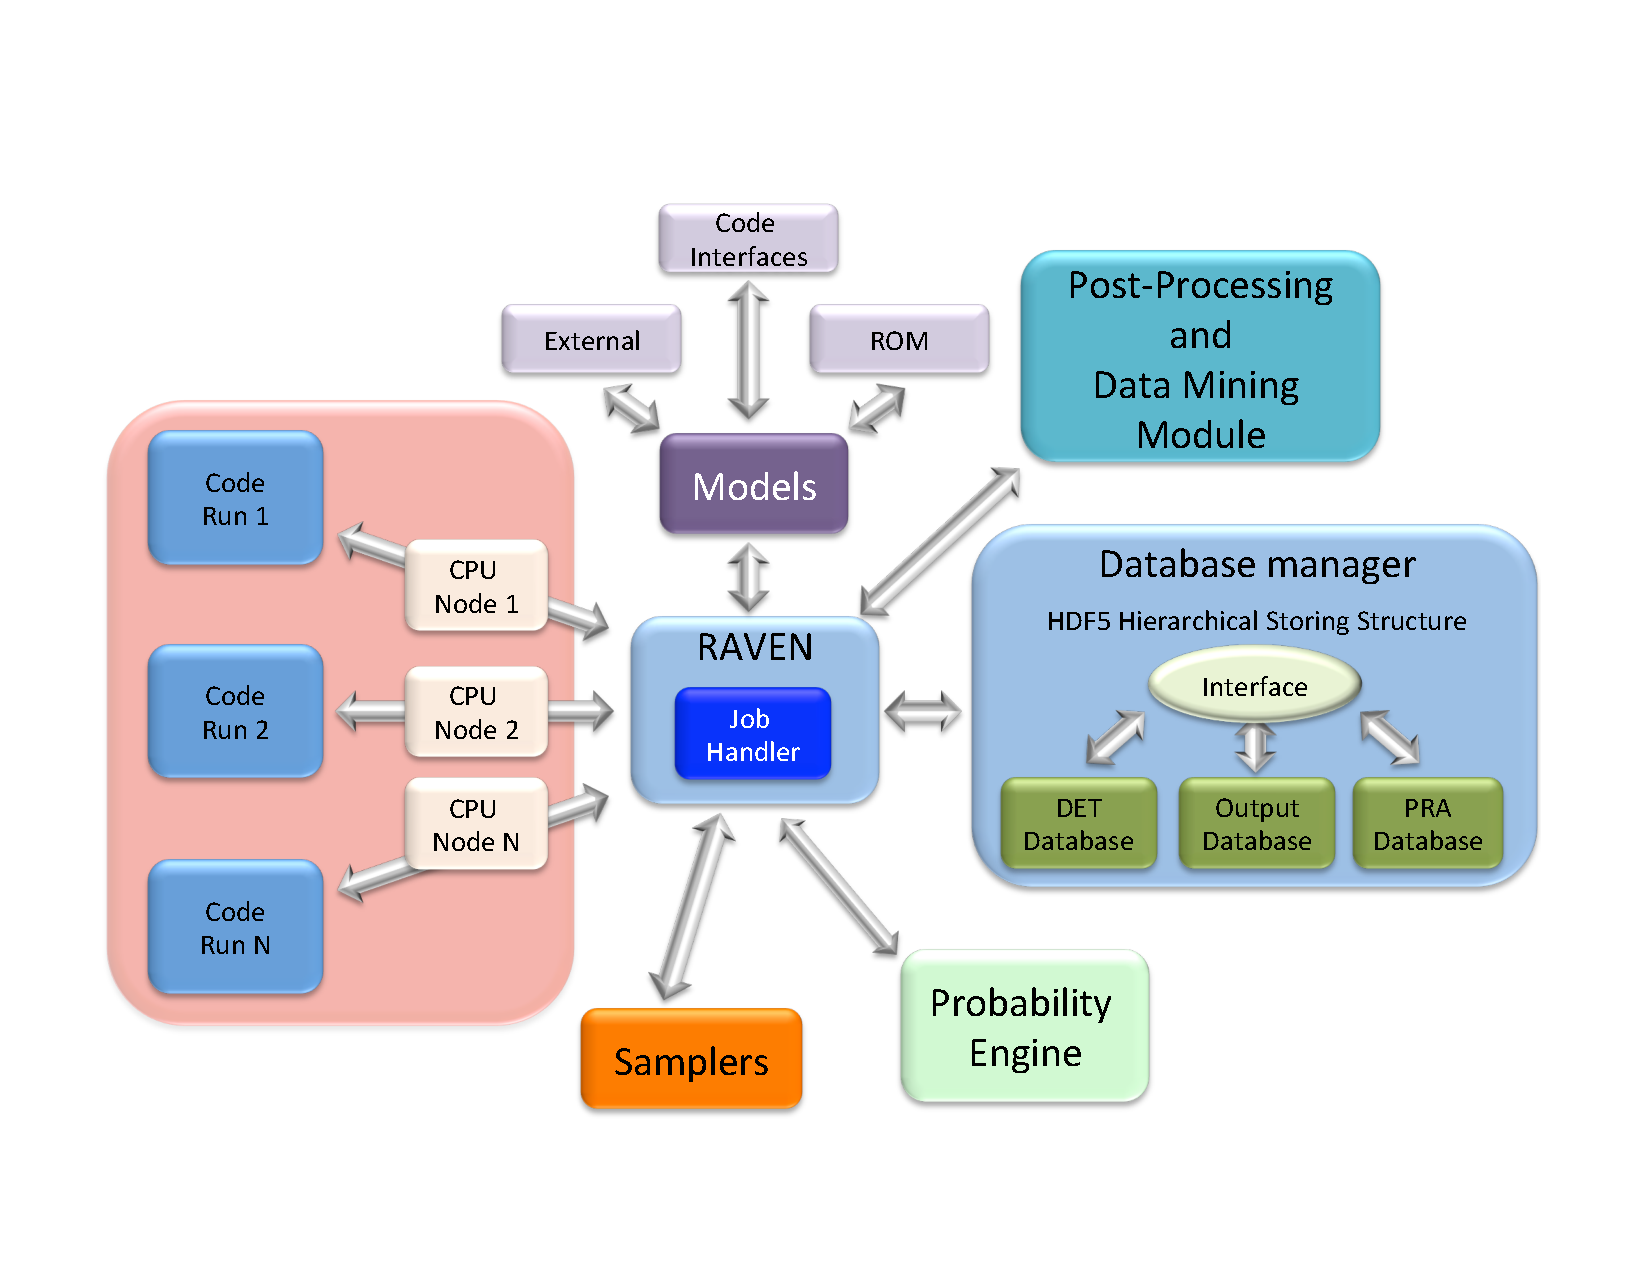
\includegraphics[scale=0.4]{raven.pdf}} 
    \caption{Overview of RAVEN statistical framework components}
    \label{fig:ravenScheme}
\end{figure}

\subsection{Ensemble-Model Capabilities}

In several cases multiple models need to interface with each other since the initial 
conditions of some are dependent on the outcomes of others. In order to face this problem 
in the RAVEN framework, a new model category (e.g., class), named EnsambleModel, was 
implemented~\cite{alfonsiEnsemble}. This class is able to assemble multiple models of 
other categories (i.e. Code, External Model, ROM), identifying the input/output connections, 
and, consequentially the order of execution and which sub-models can be executed in parallel. 
 
\begin{figure}
    \centering
    \centerline{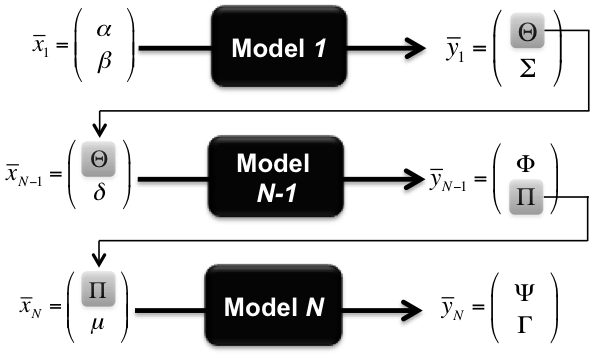
\includegraphics[scale=0.7]{LinearEnsemble.png}} 
    \caption{Example of an EnsembleModel constituted by 3 sequential sub-models.}
    \label{fig:exampleEnsembleModel}
\end{figure}
 
Figure~\ref{fig:exampleEnsembleModel} reports an example of an EnsembleModel that is constituted by 
3 sub-models (ROMs, Codes, or External Models). As it can be noticed:

\begin{itemize}
  \item The Model 2 is connected with the Model 1 through the variable $\Theta$ (Model 1 output and Model 2 input);
  \item The Model 3 is connected with the Model 2 through the variable $\Pi$ (Model 2 output and Model 3 input);
\end{itemize}

In this case, the EnsembleModel is going to drive the execution of all the sub-models in a serial sequence, 
since each model (except the Model 1) is dependent on one of the outcomes of previously executed.
In several cases, the input of a model depends on the output of another model whose input is the output 
of the initial model. In this situation, the system of equation is non-linear and an iterative solution 
procedure needs to be employed. The EnsembleModel entity in RAVEN is able to detect the non-linearity of 
the sub-models’ assembling and activate the non-linear solver: an iterative scheme. 

Figure~\ref{fig:exampleEnsembleModelNonLinear} shows an example 
of when the EnsembleModel entity activates the iteration scheme, which ends when the residue norm 
(between an iteration and the other) falls below a certain input-defined tolerance.

 \begin{figure}
    \centering
    \centerline{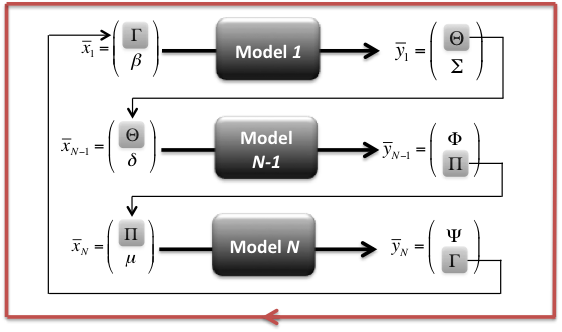
\includegraphics[scale=0.8]{NonLinearEnsemble.png}} 
    \caption{EnsembleModel resolving in a non-linear system of equations – Numerical iterations.}
    \label{fig:exampleEnsembleModelNonLinear}
\end{figure}

In RAVEN all the models’ outputs (e.g., whatever code output, etc.) are collected in internal containers 
(named DataObjects) that are aimed to store time-series and input/output data relations in a standardized 
fashion; in this way, the communication of the output information among different entities (i.e., Models) 
can be completely agnostic with respect to the particular type of output generated by a 
model.

In our multi-unit PRA analysis, we employ the RAVEN EnsembleModel feature in order to link the actual
plant models and create a link between sampled parameters and plant status in a coherent way 
(see Section~\ref{sec:RISMC_MU_modeling}).

 